\documentclass[journal]{IEEEtran}

\usepackage[T1]{fontenc}
\usepackage[utf8]{inputenc}

\usepackage{cite}
\usepackage{amsmath,amssymb}
\interdisplaylinepenalty=2500
\usepackage{bm}
\usepackage{graphicx}
\usepackage{url}
\usepackage{xcolor}
\usepackage{tikz}

\usetikzlibrary{
    arrows.meta,
    positioning,
    fit,
    calc
}

% Optional: keep only if algorithms will be included later
% \usepackage[ruled,linesnumbered]{algorithm2e}

% ------------------------------------------------------------
% Colors used by the methodology figures
% ------------------------------------------------------------
\definecolor{mygreen}{RGB}{84,130,53}
\definecolor{execBlue}{RGB}{0,51,102}
\definecolor{lookBlue}{RGB}{219,238,255}
\definecolor{textGray}{RGB}{70,70,70}
\definecolor{forBlue}{RGB}{40,105,170}
\definecolor{forBlueLight}{RGB}{222,235,247}
\definecolor{doeGreen}{RGB}{80,140,80}
\definecolor{doeGreenLight}{RGB}{226,239,218}
\definecolor{softGray}{RGB}{245,245,245}
\definecolor{darkGray}{RGB}{70,70,70}

% Colors used in the voltage-limit figure
\definecolor{voltBlue}{RGB}{32,92,168}
\definecolor{voltBlueFill}{RGB}{210,229,244}
\definecolor{voltOrange}{RGB}{218,126,35}
\definecolor{voltRed}{RGB}{190,52,62}
\definecolor{voltTeal}{RGB}{64,157,148}
\definecolor{voltGray}{RGB}{70,70,70}

\usepackage{booktabs}
\usepackage{array}
\usepackage{tabularx}
\usepackage{makecell}
\usepackage{colortbl}

% Colors for the comparison table
\definecolor{tabBlue}{RGB}{49,102,176}
\definecolor{tabOrange}{RGB}{224,138,30}
\definecolor{tabHeader}{RGB}{229,236,246}
\definecolor{tabStripe}{RGB}{247,249,252}
\definecolor{tabHighlight}{RGB}{255,242,219}

% Table symbols
\newcommand{\fullmark}{\textcolor{tabBlue}{\(\bullet\)}}
\newcommand{\partmark}{\textcolor{tabOrange}{\(\circ\)}}
\newcommand{\nomark}{\textcolor{black!45}{--}}

% ------------------------------------------------------------
% Review proposals (Ignacio): a proposed rewrite is kept as a
% colored paragraph next to the untouched original, following
% Tulio's review convention. Remove/neutralize \propuesta before
% submission. Muted steel blue color used.
% ------------------------------------------------------------
\definecolor{propColor}{RGB}{18,84,140}
\newcommand{\propuesta}[1]{\textcolor{propColor}{#1}}

\title{DSO-Led Fair Dynamic Operating Envelopes for Aggregator-Level and Prosumer-Level Flexibility Coordination}

\author{
Tulio~Coura,~\IEEEmembership{Student~Member,~IEEE},
Ignacio~Pérez~Ortiz,
Luis~Gutiérrez,~\IEEEmembership{Member,~IEEE},
and~Mariana~Resener,~\IEEEmembership{Senior~Member,~IEEE}
%
\thanks{Tulio Coura and Mariana Resener are with Simon Fraser University,
Surrey, BC, Canada
(e-mail: \{thc22, mresener\}@sfu.ca).}
%
\thanks{Ignacio Pérez Ortiz and Luis Gutiérrez are with Universidad Adolfo
Ibáñez, Santiago, Chile
(e-mail: ignacio.perez.o@edu.uai.cl; luis.gutierrez.l@ieee.org).}
}

\begin{document}

\markboth{IEEE Transactions on Smart Grid,~Vol.~XX, No.~X, Month~2026}%
{Coura \MakeLowercase{\textit{et al.}}: DSO-Led Fair Dynamic Operating Envelopes...}

\maketitle

\begin{abstract}
% Abstract to be written.
\end{abstract}

\begin{IEEEkeywords}
distributed energy resources, dynamic operating envelopes, feasible operating region, aggregators, distribution systems, fairness.
\end{IEEEkeywords}

\IEEEpeerreviewmaketitle

\section{Introduction}
\label{sec:introduction}

\IEEEPARstart{T}{he} growth of distributed energy resources (DERs), including rooftop photovoltaic (PV) systems and battery energy storage systems (BESSs), creates new opportunities for distribution networks to provide flexibility to the upstream grid \cite{iea2022}. Aggregators enable this participation by coordinating small-scale resources into portfolios for energy, ancillary services, and local flexibility markets \cite{carreiro2017,miah2026ancillary}. In distribution systems with multiple aggregators, flexibility provision also requires coordination among actors whose objectives need not coincide. Local prosumer operation, aggregator portfolio objectives, distribution system operator (DSO) security requirements, and upstream service requests must be reconciled. Prosumers operate their PV and BESS assets to serve their own consumption first. What a distribution network can offer upstream is therefore a residual: the capability that remains once local operation is committed. Aggregating device-level capabilities does not guarantee that the resulting portfolio flexibility can be delivered at the point of common coupling (PCC). The response available at the PCC depends on network operating conditions and, for BESSs, on the energy state established by previous operation. A network-level representation is therefore needed to assess the grid-feasible flexibility available at the PCC.

Region-based methods provide such a representation through the feasible operating region (FOR). The FOR describes the set of active--reactive power exchanges that a distribution system can deliver at the PCC without violating network or device constraints. Early studies established $P$--$Q$ interface regions for transmission--distribution coordination \cite{capitanescu2018,silva2018flexibility}. Random-sampling and OPF-based methods for computing these regions were compared and validated in \cite{contreras2021for}. Subsequent work examined how DER capabilities, integrated MV--LV constraints, and detailed network representations affect the size and shape of these regions \cite{riaz2022characterisation,gutierrez2021}, and robust methods have characterized the capability area under operational uncertainty \cite{kalantar2020reserve}. More recent region-based formulations have considered unbalanced multiphase networks \cite{forUnbalancedPV2025} and time-varying operating regions at feeder and end-user connection points \cite{lankeshwara2024operatingregions}. These formulations capture how flexibility changes with network and operating conditions. When BESSs are included, operating periods are also linked because charging and discharging decisions modify the state of charge and change the flexibility available later.

This dependence has motivated multi-period and online approaches to flexibility characterization. Aggregation and fair disaggregation of DER flexibility were formalized with zonotopic sets in \cite{muller2019zonotopes}. Chen \emph{et al.} represented feasible aggregate power trajectories with disaggregation guarantees and incorporated them into a model-predictive control framework \cite{chen2020aggregate}. Chen and Li developed multi-period active-power intervals and $P$--$Q$ regions with disaggregation guarantees \cite{chen2021aro}, while Wen \emph{et al.} characterized and optimized time-coupled flexibility under distribution-network security constraints \cite{wen2023temporal,wen2025timecoupled}. At the TSO--DSO interface, L{\'o}pez \emph{et al.} developed multi-period flexibility regions conditioned on deployed flexibility \cite{lopez2022multiperiod}, and online methods have used dispatch feedback to update future portfolio flexibility \cite{wang2025onlinehierarchical}. These approaches capture important links between present operation and future flexibility. The setting considered here introduces a specific operational sequence: local operation is first established through a network-constrained self-consumption dispatch, and the BESS actions implemented in that dispatch determine the state from which the next PCC FOR is constructed. In this way, upstream flexibility is a residual quantity. It is evaluated from the state the local dispatch leaves behind, not from an independently assumed BESS state.

A dispatch-conditioned PCC FOR determines the flexibility that remains available to the upstream grid, but it does not determine how a selected response should be realized by the actors behind the PCC. Operating-envelope methods provide time-varying active-power limits for DER owners and aggregators \cite{petrou2021,liu2022}, with extensions to $P$--$Q$ operating regions \cite{zabihinia2022pqdoe,lankeshwara2024operatingregions} and allocation schemes based on proportional, technical, and equity-based criteria at the prosumer level \cite{petrou2020weighted,alam2023,gao2025equitablepq}. These allocation schemes respond to earlier evidence that network location alone creates unequal treatment among prosumers \cite{tonkoski2011curtailment,lusis2020fairness} and that reactive-power control can reduce this inequality \cite{gebbran2021voltvar}. For systems with multiple aggregators, network-secure operating regions and coordination mechanisms have also been developed to manage network access and shared constraints \cite{russell2024networksecure,chen2024dera,jiang2025bargaining}, and fairness has been considered in time-dependent $P$--$Q$ flexibility provision \cite{kryonidis2025fair}. Reactive-power flexibility has also been used to improve the fairness of active-power export allocations, although at the prosumer level only \cite{lukac2026reactivefair}. These methods primarily determine permissible participant operation, network access, or flexibility allocation. The activation problem considered here starts from a different decision point: an upstream service request has selected a specific operating point from the PCC FOR, and coordinated participant setpoints must reproduce that exchange while respecting the distribution network. With multiple aggregators, this realization also introduces two allocation levels, first among aggregators and then among the prosumers within each aggregator. Fairness at both levels is an operational requirement rather than a design preference. A DSO-led scheme should treat competing aggregators without discrimination, and repeated activations should not concentrate effort on prosumers at electrically favorable network locations.

\begin{table}[t]
\centering
\caption{Comparison With the Closest Region- and Envelope-Based Methods}
\label{tab:comparison}
\scriptsize
\setlength{\tabcolsep}{3.5pt}
\renewcommand{\arraystretch}{1.25}
\begin{tabular}{@{}lcccccc@{}}
\toprule
 & \makecell{$P$--$Q$\\PCC\\region} & \makecell{Dispatch-\\cond.\\rolling} & \makecell{Multiple\\aggreg.} & \makecell{Two-level\\fairness} & \makecell{Unbal.\\MV--LV} & \makecell{Activation\\guarantee} \\
\midrule
Chen \emph{et al.}~\cite{chen2020aggregate} & \fullmark & \partmark & \nomark & \nomark & \partmark & \fullmark \\
Lankeshwara \emph{et al.}~\cite{lankeshwara2024operatingregions} & \fullmark & \partmark & \nomark & \nomark & \partmark & \fullmark \\
Russell \emph{et al.}~\cite{russell2024networksecure} & \fullmark & \nomark & \partmark & \nomark & \partmark & \fullmark \\
Jiang and Guo~\cite{jiang2025bargaining} & \nomark & \nomark & \fullmark & \partmark & \nomark & \fullmark \\
Gao \emph{et al.}~\cite{gao2025equitablepq} & \partmark & \nomark & \nomark & \partmark & \partmark & \fullmark \\
Luka\v{c} \emph{et al.}~\cite{lukac2026reactivefair} & \partmark & \nomark & \nomark & \partmark & \partmark & \fullmark \\
\rowcolor{tabHighlight}
\textbf{This paper} & \fullmark & \fullmark & \fullmark & \fullmark & \fullmark & \fullmark \\
\bottomrule
\multicolumn{7}{@{}l@{}}{\rule{0pt}{2.2ex}\fullmark\ addressed \quad \partmark\ partial \quad \nomark\ not considered}\\
\end{tabular}
\end{table}

The reviewed formulations therefore address complementary parts of the flexibility-provision problem, but they do not jointly establish the operational chain considered in this work. Table~\ref{tab:comparison} positions the proposed framework against the closest region- and envelope-based methods. In particular, the local dispatch that determines the current BESS state must be linked to the flexibility offered in the next interval, and a selected point from that offer must be linked to its network-feasible realization across multiple aggregators and prosumers. An operationally consistent PCC offer should be network-feasible when constructed, reachable from the state established by the implemented dispatch, and realizable by the participating resources when activated. Without these links, an offered region may be feasible for an assumed operating state but unavailable after the actual BESS operation, or a valid PCC request may lack a corresponding network-feasible and fair participant-level dispatch.

Accordingly, this paper develops a DSO-led rolling-horizon framework that connects network-constrained self-consumption, dispatch-conditioned PCC flexibility, and two-level fair activation across multiple aggregators and their prosumers. At each rolling step, a network-constrained self-consumption problem establishes local operation and determines the BESS actions implemented in the current interval. The resulting state of charge is carried forward to construct the next PCC FOR. Once an upstream service request selects an operating point from this region, the required deviation from the self-consumption baseline is coordinated first among aggregators and then among their prosumers while preserving network feasibility. The main contributions are as follows:

\begin{enumerate}
\item A rolling-horizon construction that quantifies the grid-feasible $P$--$Q$ flexibility remaining at the PCC after prosumer self-consumption is committed. The network-constrained dispatch fixes the BESS state from which the next-interval region is built, so every offered operating point is reachable from implemented operation under the adopted three-phase MV--LV formulation.

\item A network-feasible hierarchical activation formulation is developed for a selected PCC operating point, with fairness enforced at two levels: first among competing aggregators and then among the prosumers within each aggregator. The formulation coordinates the required deviation from the self-consumption baseline while preserving the requested PCC exchange and distribution-network constraints.

\item A comprehensive operational assessment quantifies the effects of dispatch commitment and two-level fairness on reachable flexibility, resource utilization, BESS throughput, and computational performance. The analysis also distinguishes the complete feeder-level PCC flexibility, which reflects the combined effect of demand, PV generation, controllable resources, and network conditions, from the controllable BESS contribution around the established distribution-system operating point.

\end{enumerate}

The remainder of this paper is organized as follows. Section~\ref{sec:method} presents the proposed rolling-horizon framework, including state propagation, the self-consumption and reachable-region formulations, and the hierarchical activation method. Section~\ref{sec:case} describes the unbalanced MV--LV test system, DER data, fairness criteria, and simulation setup. Section~\ref{sec:results} evaluates the reachable $P$--$Q$ regions, service activation, resource allocation, and computational performance. Section~\ref{sec:concl} summarizes the main findings and concludes the paper.


% =====================================================================
\section{Rolling-Horizon Coordination Framework for Reachable FORs}
\label{sec:method}


The proposed framework coordinates the flexibility of prosumer-owned PV and BESS units. Every 30 minutes, the DSO computes the feasible operating region (FOR) of active and reactive power at the distribution network PCC. Each operating point within the FOR reflects the self-consumption dispatch implemented by the prosumers and is therefore operationally achievable.

In this work, \textit{self-consumption} denotes the use of local PV and BESS resources to meet household demand before providing system flexibility. \textit{Flexibility} denotes the residual active and reactive power capability available at the PCC after this dispatch is committed. A \textit{rolling-horizon} scheme links both stages by re-optimizing a 48-slot window every half-hour.

At each rolling step, the methodology solves two optimization problems in sequence. Problem 1 (P1) computes a network-constrained self-consumption dispatch and commits the current BESS actions. The batteries discharge during PV deficits and charge during PV surpluses, minimizing prosumer--network power exchanges and determining the battery states entering the next interval.

Problem~2 (P2) fixes the BESS actions committed by P1 and applies a directional optimal power flow (OPF) to compute the FOR for the next interval. The 48 half-hourly FORs describe what the DN can deliver at the PCC throughout the day. The complete process is summarized in Fig.~\ref{fig:coordination_concept} and detailed below.

\begin{figure}[h!]
\centering
\resizebox{\columnwidth}{!}{%
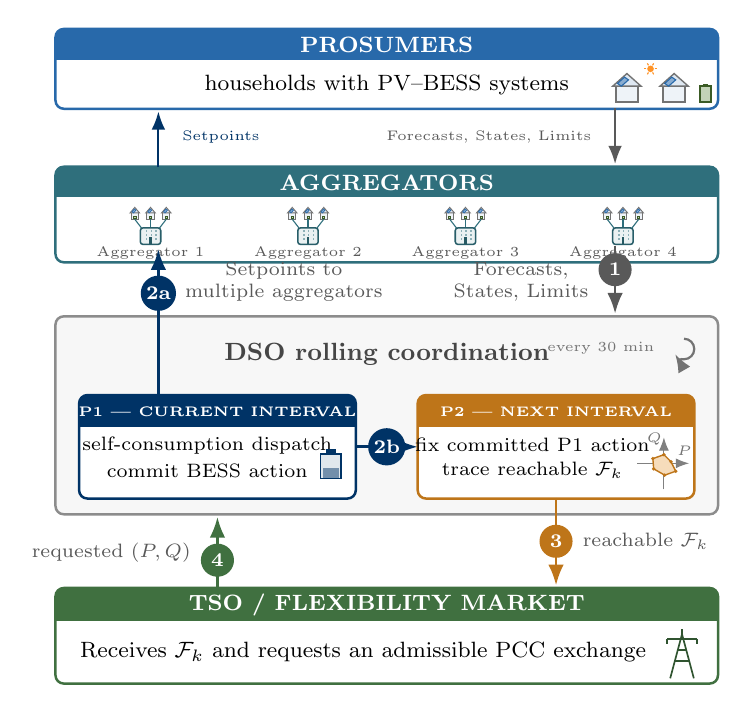
\begin{tikzpicture}[
    font=\footnotesize,
    >=Latex,
    card/.style={rounded corners=3pt, fill=white, inner sep=0pt},
    lbl/.style={font=\scriptsize, text=black!65, align=center, inner sep=1.5pt},
    badge/.style={circle, text=white, inner sep=1pt, minimum size=0.42cm,
        font=\scriptsize\bfseries},
    flow/.style={->, line width=1.0pt},
]
\definecolor{figOrange}{RGB}{224,138,30}
\definecolor{figTeal}{RGB}{47,111,124}

% --------------------------- prosumers card ---------------------------
\node[card, minimum width=8.4cm, minimum height=1.0cm] (resources) at (0,0) {};
\begin{scope}
  \clip[rounded corners=3pt] (resources.south west) rectangle (resources.north east);
  \fill[forBlue] ([yshift=-0.40cm]resources.north west) rectangle (resources.north east);
\end{scope}
\draw[rounded corners=3pt, line width=0.9pt, forBlue]
  (resources.south west) rectangle (resources.north east);
\node[font=\footnotesize\bfseries, text=white] at (0,0.30)
  {PROSUMERS};
\node[font=\footnotesize] at (0,-0.20)
  {households with PV--BESS systems};
% prosumer community: two PV houses, battery, sun
\foreach \cx in {3.05,3.65}{%
  \draw[line width=0.5pt, draw=black!55, fill=forBlue!8]
    (\cx-0.14,-0.42) rectangle (\cx+0.14,-0.22);
  \draw[line width=0.5pt, draw=black!55, fill=forBlue!15]
    (\cx-0.18,-0.22) -- (\cx,-0.06) -- (\cx+0.18,-0.22) -- cycle;
  \draw[line width=0.4pt, draw=forBlue, fill=forBlue!55]
    (\cx-0.12,-0.185) -- (\cx-0.03,-0.105) -- (\cx+0.02,-0.14)
    -- (\cx-0.07,-0.22) -- cycle;}
\draw[line width=0.5pt, draw=mygreen!70!black, fill=mygreen!35]
  (3.98,-0.42) rectangle (4.12,-0.22);
\fill[mygreen!70!black] (4.02,-0.22) rectangle (4.08,-0.19);
\fill[orange!85] (3.35,0.0) circle (0.042);
\foreach \ang in {0,60,120,180,240,300}{%
  \draw[orange!85, line width=0.4pt]
    ([shift={(\ang:0.052)}]3.35,0.0) -- ([shift={(\ang:0.08)}]3.35,0.0);}

% ------------------------- aggregators layer --------------------------
\node[
    card,
    minimum width=8.4cm,
    minimum height=1.20cm
] (agg) at (0,-1.85) {};

\begin{scope}
  \clip[rounded corners=3pt]
    (agg.south west) rectangle (agg.north east);
  \fill[figTeal]
    ([yshift=-0.38cm]agg.north west) rectangle (agg.north east);
\end{scope}

\draw[
    rounded corners=3pt,
    line width=0.9pt,
    figTeal
]
(agg.south west) rectangle (agg.north east);

\node[
    font=\footnotesize\bfseries,
    text=white
] at (0,-1.45)
{AGGREGATORS};

% =========================================================
% Aggregator company 1
% =========================================================
\begin{scope}[shift={(-3.00,-2.03)}]

  \foreach \x in {-0.20,0,0.20}{
    % house body
    \draw[line width=0.35pt, draw=black!55, fill=forBlue!8]
      (\x-0.045,0.12) rectangle (\x+0.045,0.20);
    % roof
    \draw[line width=0.35pt, draw=black!55, fill=forBlue!15]
      (\x-0.06,0.20) -- (\x,0.27) -- (\x+0.06,0.20) -- cycle;
    % PV panel
    \draw[line width=0.25pt, draw=forBlue, fill=forBlue!55]
      (\x-0.035,0.215) -- (\x-0.005,0.25) -- (\x+0.015,0.235)
      -- (\x-0.015,0.20) -- cycle;
    % battery inside house
    \draw[line width=0.2pt, draw=mygreen!70!black, fill=mygreen!35]
      (\x-0.013,0.132) rectangle (\x+0.013,0.162);
  }

  % connections
  \draw[figTeal, line width=0.4pt] (-0.20,0.12) -- (-0.10,-0.01);
  \draw[figTeal, line width=0.4pt] (0,0.12) -- (0,-0.01);
  \draw[figTeal, line width=0.4pt] (0.20,0.12) -- (0.10,-0.01);

  % building
  \draw[
      rounded corners=1pt,
      line width=0.55pt,
      draw=figTeal!85!black,
      fill=figTeal!10
  ]
  (-0.13,-0.20) rectangle (0.13,0.01);

  % windows
  \foreach \x in {-0.06,0.00,0.06}{
    \foreach \y in {-0.14,-0.09,-0.04}{
      \fill[figTeal!55] (\x,\y) rectangle ++(0.018,0.018);
    }
  }

  % door
  \fill[figTeal!80!black] (-0.018,-0.20) rectangle (0.018,-0.11);

  % label
  \node[font=\tiny, text=black!65, align=center] at (0,-0.31)
  {Aggregator 1};

\end{scope}

% =========================================================
% Aggregator company 2
% =========================================================
\begin{scope}[shift={(-1.00,-2.03)}]

  \foreach \x in {-0.20,0,0.20}{
    \draw[line width=0.35pt, draw=black!55, fill=forBlue!8]
      (\x-0.045,0.12) rectangle (\x+0.045,0.20);
    \draw[line width=0.35pt, draw=black!55, fill=forBlue!15]
      (\x-0.06,0.20) -- (\x,0.27) -- (\x+0.06,0.20) -- cycle;
    \draw[line width=0.25pt, draw=forBlue, fill=forBlue!55]
      (\x-0.035,0.215) -- (\x-0.005,0.25) -- (\x+0.015,0.235)
      -- (\x-0.015,0.20) -- cycle;
    \draw[line width=0.2pt, draw=mygreen!70!black, fill=mygreen!35]
      (\x-0.013,0.132) rectangle (\x+0.013,0.162);
  }

  \draw[figTeal, line width=0.4pt] (-0.20,0.12) -- (-0.10,-0.01);
  \draw[figTeal, line width=0.4pt] (0,0.12) -- (0,-0.01);
  \draw[figTeal, line width=0.4pt] (0.20,0.12) -- (0.10,-0.01);

  \draw[
      rounded corners=1pt,
      line width=0.55pt,
      draw=figTeal!85!black,
      fill=figTeal!10
  ]
  (-0.13,-0.20) rectangle (0.13,0.01);

  \foreach \x in {-0.06,0.00,0.06}{
    \foreach \y in {-0.14,-0.09,-0.04}{
      \fill[figTeal!55] (\x,\y) rectangle ++(0.018,0.018);
    }
  }

  \fill[figTeal!80!black] (-0.018,-0.20) rectangle (0.018,-0.11);

  \node[font=\tiny, text=black!65, align=center] at (0,-0.31)
  {Aggregator 2};

\end{scope}

% =========================================================
% Aggregator company 3
% =========================================================
\begin{scope}[shift={(1.00,-2.03)}]

  \foreach \x in {-0.20,0,0.20}{
    \draw[line width=0.35pt, draw=black!55, fill=forBlue!8]
      (\x-0.045,0.12) rectangle (\x+0.045,0.20);
    \draw[line width=0.35pt, draw=black!55, fill=forBlue!15]
      (\x-0.06,0.20) -- (\x,0.27) -- (\x+0.06,0.20) -- cycle;
    \draw[line width=0.25pt, draw=forBlue, fill=forBlue!55]
      (\x-0.035,0.215) -- (\x-0.005,0.25) -- (\x+0.015,0.235)
      -- (\x-0.015,0.20) -- cycle;
    \draw[line width=0.2pt, draw=mygreen!70!black, fill=mygreen!35]
      (\x-0.013,0.132) rectangle (\x+0.013,0.162);
  }

  \draw[figTeal, line width=0.4pt] (-0.20,0.12) -- (-0.10,-0.01);
  \draw[figTeal, line width=0.4pt] (0,0.12) -- (0,-0.01);
  \draw[figTeal, line width=0.4pt] (0.20,0.12) -- (0.10,-0.01);

  \draw[
      rounded corners=1pt,
      line width=0.55pt,
      draw=figTeal!85!black,
      fill=figTeal!10
  ]
  (-0.13,-0.20) rectangle (0.13,0.01);

  \foreach \x in {-0.06,0.00,0.06}{
    \foreach \y in {-0.14,-0.09,-0.04}{
      \fill[figTeal!55] (\x,\y) rectangle ++(0.018,0.018);
    }
  }

  \fill[figTeal!80!black] (-0.018,-0.20) rectangle (0.018,-0.11);

  \node[font=\tiny, text=black!65, align=center] at (0,-0.31)
  {Aggregator 3};

\end{scope}

% =========================================================
% Aggregator company 4
% =========================================================
\begin{scope}[shift={(3.00,-2.03)}]

  \foreach \x in {-0.20,0,0.20}{
    \draw[line width=0.35pt, draw=black!55, fill=forBlue!8]
      (\x-0.045,0.12) rectangle (\x+0.045,0.20);
    \draw[line width=0.35pt, draw=black!55, fill=forBlue!15]
      (\x-0.06,0.20) -- (\x,0.27) -- (\x+0.06,0.20) -- cycle;
    \draw[line width=0.25pt, draw=forBlue, fill=forBlue!55]
      (\x-0.035,0.215) -- (\x-0.005,0.25) -- (\x+0.015,0.235)
      -- (\x-0.015,0.20) -- cycle;
    \draw[line width=0.2pt, draw=mygreen!70!black, fill=mygreen!35]
      (\x-0.013,0.132) rectangle (\x+0.013,0.162);
  }

  \draw[figTeal, line width=0.4pt] (-0.20,0.12) -- (-0.10,-0.01);
  \draw[figTeal, line width=0.4pt] (0,0.12) -- (0,-0.01);
  \draw[figTeal, line width=0.4pt] (0.20,0.12) -- (0.10,-0.01);

  \draw[
      rounded corners=1pt,
      line width=0.55pt,
      draw=figTeal!85!black,
      fill=figTeal!10
  ]
  (-0.13,-0.20) rectangle (0.13,0.01);

  \foreach \x in {-0.06,0.00,0.06}{
    \foreach \y in {-0.14,-0.09,-0.04}{
      \fill[figTeal!55] (\x,\y) rectangle ++(0.018,0.018);
    }
  }

  \fill[figTeal!80!black] (-0.018,-0.20) rectangle (0.018,-0.11);

  \node[font=\tiny, text=black!65, align=center] at (0,-0.31)
  {Aggregator 4};

\end{scope}


% --------------------------- DSO container ----------------------------
\node[card, fill=black!3, minimum width=8.4cm, minimum height=2.5cm]
  (dso) at (0,-4.40) {};
\draw[rounded corners=3pt, line width=0.9pt, black!45]
  (dso.south west) rectangle (dso.north east);
\node[font=\small\bfseries, text=darkGray] at (0,-3.63)
  {DSO rolling coordination};
\draw[black!55, line width=0.8pt, ->]
  ([shift={(110:0.13)}]3.82,-3.55) arc[start angle=90, end angle=-150, radius=0.13];
\node[font=\tiny, text=black!55, anchor=east] at (3.52,-3.55) {every 30 min};

% ------------------------------ P1 card -------------------------------
\node[card, minimum width=3.5cm, minimum height=1.3cm] (p1) at (-2.15,-4.80) {};
\begin{scope}
  \clip[rounded corners=3pt] (p1.south west) rectangle (p1.north east);
  \fill[execBlue] ([yshift=-0.4cm]p1.north west) rectangle (p1.north east);
\end{scope}
\draw[rounded corners=3pt, line width=0.9pt, execBlue]
  (p1.south west) rectangle (p1.north east);
\node[font=\tiny\bfseries, text=white] at (-2.15,-4.35)
  {P1 --- CURRENT INTERVAL};
\node[font=\scriptsize] at (-2.28,-4.78) {self-consumption dispatch};
\node[font=\scriptsize] at (-2.28,-5.10) {commit BESS action};
% battery glyph
\draw[line width=0.5pt, draw=execBlue, fill=execBlue!12]
  (-0.84,-5.20) rectangle (-0.58,-4.89);
\fill[execBlue] (-0.77,-4.89) rectangle (-0.65,-4.83);
\fill[execBlue!55] (-0.81,-5.20) rectangle (-0.61,-5.07);

% ------------------------------ P2 card -------------------------------
\node[card, minimum width=3.5cm, minimum height=1.3cm] (p2) at (2.15,-4.80) {};
\begin{scope}
  \clip[rounded corners=3pt] (p2.south west) rectangle (p2.north east);
  \fill[figOrange!85!black] ([yshift=-0.4cm]p2.north west) rectangle (p2.north east);
\end{scope}
\draw[rounded corners=3pt, line width=0.9pt, figOrange!85!black]
  (p2.south west) rectangle (p2.north east);
\node[font=\tiny\bfseries, text=white] at (2.15,-4.35)
  {P2 --- NEXT INTERVAL};
\node[font=\scriptsize] at (1.85,-4.78) {fix committed P1 action};
\node[font=\scriptsize] at (1.85,-5.10) {trace reachable $\mathcal F_k$};
% mini FOR chart: P-Q axes and vertex dots
\draw[->, black!50, line width=0.4pt] (3.18,-5.01) -- (3.84,-5.01);
\draw[->, black!50, line width=0.4pt] (3.52,-5.34) -- (3.52,-4.68);
\node[font=\tiny, text=black!55] at (3.78,-4.85) {$P$};
\node[font=\tiny, text=black!55] at (3.40,-4.70) {$Q$};
\fill[figOrange!30, draw=figOrange!85!black, line width=0.5pt]
  (3.52,-4.90) -- (3.61,-4.99) -- (3.67,-5.11) -- (3.53,-5.16)
  -- (3.39,-5.08) -- (3.38,-4.95) -- cycle;
\foreach \vx/\vy in {3.52/-4.90, 3.61/-4.99, 3.67/-5.11, 3.53/-5.16,
                     3.39/-5.08, 3.38/-4.95}{%
  \fill[figOrange!85!black] (\vx,\vy) circle (0.024);}

% ------------------------------ TSO card ------------------------------
\node[card, minimum width=8.4cm, minimum height=1.2cm] (tso) at (0,-7.20) {};
\begin{scope}
  \clip[rounded corners=3pt] (tso.south west) rectangle (tso.north east);
  \fill[doeGreen!80!black] ([yshift=-0.42cm]tso.north west) rectangle (tso.north east);
\end{scope}
\draw[rounded corners=3pt, line width=0.9pt, doeGreen!80!black]
  (tso.south west) rectangle (tso.north east);
\node[font=\footnotesize\bfseries, text=white] at (0,-6.81)
  {TSO / FLEXIBILITY MARKET};
\node[font=\footnotesize] at (-0.3,-7.41)
  {Receives $\mathcal F_k$ and requests an admissible PCC exchange};
% transmission tower glyph
\draw[doeGreen!60!black, line width=0.6pt]
  (3.60,-7.74) -- (3.75,-7.18) -- (3.90,-7.74);
\draw[doeGreen!60!black, line width=0.5pt] (3.66,-7.52) -- (3.84,-7.52);
\draw[doeGreen!60!black, line width=0.5pt] (3.69,-7.38) -- (3.81,-7.38);
\draw[doeGreen!60!black, line width=0.7pt] (3.56,-7.24) -- (3.94,-7.24);
\draw[doeGreen!60!black, line width=0.5pt] (3.56,-7.24) -- (3.56,-7.30);
\draw[doeGreen!60!black, line width=0.5pt] (3.94,-7.24) -- (3.94,-7.30);
\draw[doeGreen!60!black, line width=0.5pt] (3.75,-7.18) -- (3.75,-7.12);

% --------------------- prosumers <-> aggregators ---------------------
% relay hop: no step number, the aggregator mediates
\draw[flow, line width=0.8pt, black!65] (2.9,-0.50) -- (2.9,-1.21);
\node[font=\tiny, text=black!65, anchor=east] at (2.72,-0.87)
  {Forecasts, States, Limits};
\draw[flow, line width=0.8pt, execBlue] (-2.9,-1.25) -- (-2.9,-0.54);
\node[font=\tiny, text=execBlue, anchor=west] at (-2.72,-0.87)
  {Setpoints};

% -------------------------- aggregators <-> DSO -----------------------
% Step 1: aggregated data to the DSO (down, right lane)
\draw[flow, black!65] (2.9,-2.25) -- (2.9,-3.11);
\node[badge, fill=black!65] at (2.9,-2.55) {1};
\node[lbl, anchor=east] at (2.62,-2.70) {Forecasts,\\States, Limits};

% Step 2a: committed setpoints back through the aggregators (up, left lane)
\draw[flow, execBlue] (-2.9,-4.15) -- (-2.9,-2.29);
\node[badge, fill=execBlue] at (-2.9,-2.85) {2a};
\node[lbl, anchor=west] at (-2.62,-2.70) {Setpoints to\\multiple aggregators};

% Step 2b: P1 action frozen in P2
\draw[flow, execBlue] (p1.east) -- (p2.west);
\node[badge, fill=execBlue] at (0,-4.80) {2b};

% --------------------------- DSO <-> TSO -----------------------------
% Step 3: reachable region to the TSO (down, right lane)
\draw[flow, figOrange!85!black] (2.15,-5.45) -- (2.15,-6.56);
\node[badge, fill=figOrange!85!black] at (2.15,-6.00) {3};
\node[lbl, anchor=west] at (2.43,-6.00) {reachable $\mathcal F_k$};

% Step 4: requested exchange back to the DSO (up, left lane)
\draw[flow, doeGreen!80!black] (-2.15,-6.60) -- (-2.15,-5.69);
\node[badge, fill=doeGreen!80!black] at (-2.15,-6.24) {4};
\node[lbl, anchor=east] at (-2.43,-6.14) {requested $(P,Q)$};

\end{tikzpicture}%
}
\caption{Rolling-horizon coordination among prosumers, aggregators, the DSO, and the TSO. Aggregators are the sole interface between prosumers and the DSO. P1 commits the current BESS action (Steps 1--2a), P2
conditions the next-interval FOR on that action (Step 2b), and the TSO requests an exchange within the offered region (Steps 3--4).}
\label{fig:coordination_concept}
\end{figure}

The DSO coordinates the process based on its network model, measurements, and OPF capability~\cite{frueh2023,petrou2021,liu2022}. In Step~1, aggregators convey prosumer forecasts, measured BESS states, and operating limits to the DSO. After solving P1, the DSO sends the first-interval BESS setpoints through the aggregators for implementation (Step~2a).

The BESS actions committed by P1 are fixed in all P2 directional solves (Step~2b), ensuring that the FOR boundary is computed from a common post-dispatch state. The DSO communicates the resulting region $\mathcal{F}_k$ to the TSO or flexibility market (Step~3). Any exchange $(P,Q)\in\mathcal{F}_k$ may be requested (Step~4), as described in Section~XX.

Both problems are built on a common prosumer, BESS, and three-phase network model adapted from the convex multi-period OPF in~\cite{gutierrez2021}. Their distinction lies in the objective functions and variables fixed in each formulation. The following subsections detail the rolling-horizon timing, common model, P1 and P2 formulations, and DN-scale implementation.

% ---------------------------------------------------------------------
\subsection{Rolling-Horizon Timing and State Propagation}
\label{ssec:timing}
% ---------------------------------------------------------------------

At each rolling step \(k\), the DSO optimizes a 24-h window of \(H=48\) half-hour slots, indexed by \(h\in\mathcal{H}=\{1,\ldots,48\}\). Slot \(h=1\) represents the current interval, and slot \(h=2\) represents the next interval.

The physical periods of the day are indexed by
\(t\in\{1,\ldots,48\}\). At step \(k\), these periods are ordered as

\[
(k,k+1,\ldots,48,1,\ldots,k-1),
\]

with the physical period corresponding to slot \(h\) given by

\begin{equation}
\label{eq:time_mapping}
t_k(h)=1+\operatorname{mod}(k+h-2,48).
\end{equation}

The first two slots couple the self-consumption dispatch and the FOR
computation. Slot \(h=1\) is the \emph{operation slot}, in which the BESS
actions obtained from P1 are committed and implemented. Slot
\(h=t^\star=2\) is the \emph{flexibility slot}, for which P2 computes the
FOR while retaining the operation-slot actions. Slots \(h\geq3\) provide
the look-ahead required to preserve intertemporal and network feasibility,
as illustrated in Figure.~\ref{fig:rolling_worm}.

Although the full window is optimized, only the slot-1 BESS charging and discharging commands, \(\widehat{P}^{b,+}_{s,1\mid k}\) and \(\widehat{P}^{b,-}_{s,1\mid k}\), are implemented. These commands determine the BESS energy entering the flexibility slot: 

\begin{equation} \label{eq:committed_state} \widehat{E}^{b}_{s,1\mid k} = E^{b}_{s,0\mid k} + \Delta t \left( \eta^{b,+}_{s}\widehat{P}^{b,+}_{s,1\mid k} - \frac{\widehat{P}^{b,-}_{s,1\mid k}} {\eta^{b,-}_{s}} \right), \qquad \forall s\in\mathcal{S}, 
\end{equation} 

where \(\Delta t=0.5\)~h. 

The committed commands are fixed in every directional solve of P2. Thus, all FOR boundary points are evaluated from the same post-dispatch energy state \(\widehat{E}^{b}_{s,1\mid k}\), ensuring reachability from the implemented P1 dispatch.

When the horizon advances, the flexibility slot of step \(k\) becomes the operation slot of step \(k+1\), since \[ t_k(2)=t_{k+1}(1). \] 

Thus, \(\widehat{E}^{b}_{s,1\mid k}\) is the energy predicted by the model at the beginning of the next rolling step. After the slot-1 commands are implemented, this prediction is replaced by the measured BESS energy: 

\begin{equation} \label{eq:state_update} E^{b}_{s,0\mid k+1} = E^{b,\mathrm{meas}}_{s}\!\left(t_k(2)\right), \qquad \forall s\in\mathcal{S}. 
\end{equation} 

This measurement-based update closes the rolling-horizon loop and accounts for deviations between the predicted and realized BESS states.

Repeating this procedure throughout the day produces the sequence

\begin{equation} \label{eq:for_sequence} \left\{ \mathcal{F}_{1}, \mathcal{F}_{2}, \ldots, \mathcal{F}_{48} \right\}, \end{equation} 

where \(\mathcal{F}_{k}\) denotes the FOR computed at step \(k\) for physical period \(t_k(2)\).


\begin{figure}[h!]
\centering
% ============================ KNOBS ============================
\def\rhScale{1.00}
\colorlet{rhExec}{execBlue}
\definecolor{rhFOR}{RGB}{224,138,30}
\colorlet{rhLook}{lookBlue}
\definecolor{rhWrap}{RGB}{233,226,214}
\colorlet{rhRegion}{rhFOR}
\colorlet{rhSun}{orange}
\colorlet{rhBatt}{mygreen}
% ===============================================================
\resizebox{\rhScale\columnwidth}{!}{%
\begin{tikzpicture}[font=\footnotesize, >=Latex,
   pcell/.style={draw=black!40, line width=0.5pt, minimum width=0.6cm,
       minimum height=0.6cm, anchor=south west, inner sep=1pt, align=center, font=\scriptsize},
   ex/.style={pcell, fill=rhExec!30, draw=rhExec, line width=0.9pt},
   fo/.style={pcell, fill=rhFOR!32, draw=rhFOR!80!black, line width=0.9pt},
   lk/.style={pcell, fill=rhLook, draw=rhExec!45},
   wk/.style={pcell, fill=rhWrap, draw=black!35},
   el/.style={anchor=south west, minimum width=0.6cm, minimum height=0.6cm, align=center}]

% ---- band 1: title ----
\node[anchor=west, font=\scriptsize\bfseries, text=textGray] at (-0.0,1.8)
   {rolling step $k=20$};

% ---- band 2: brace + reading key ----
\draw[line width=0.6pt, draw=black!45] (0,1.1) -- (0,1.2) -- (8.0,1.2) -- (8.0,1.1);
\node[font=\scriptsize, text=textGray, above] at (4.0,1.2)
   {planning window: 48 slots $h$; cell numbers = physical period $t_{20}(h)$ of~\eqref{eq:time_mapping}};

% ---- band 3: h-axis markers (one row, staggered x) ----
\node[font=\tiny\bfseries, text=rhExec] at (0.30,0.84) {$h{=}1$};
\node[font=\tiny\bfseries, text=rhFOR!85!black] at (1.20,0.84) {$h{=}2{=}t^\star$};
\node[font=\tiny, text=black!55] at (5.06,0.84) {$h{=}30$};
\node[font=\tiny, text=black!55] at (7.70,0.84) {$h{=}48$};

% ---- band 4: the slot strip ----
\node[ex] at (0.00,0) {20};
\node[fo] at (0.66,0) {21};
\node[lk] at (1.32,0) {22};
\node[lk] at (1.98,0) {23};
\node[el] at (2.64,0) {$\cdots$};
\node[lk] at (3.30,0) {47};
\node[lk] at (3.96,0) {48};

\draw[dashed, line width=1pt, draw=rhFOR!85!black] (4.69,-0.10) -- (4.69,0.70);
\node[font=\tiny, text=rhFOR!85!black] at (4.69,-0.28) {midnight};

\node[wk] at (4.76,0) {1};
\node[wk] at (5.42,0) {2};
\node[wk] at (6.08,0) {3};
\node[el] at (6.74,0) {$\cdots$};
\node[wk] at (7.40,0) {19};

% ---- band 5: P1 / P2 flows and the two mini-scenes ----
\draw[->, rhExec, line width=0.8pt] (0.30,-1.10) -- (0.30,-0.05);
\node[font=\tiny\bfseries, text=rhExec, anchor=east] at (0.05,-0.58) {P1};
\draw[->, rhFOR!85!black, line width=0.8pt] (0.96,-0.05) -- (2.15,-0.80);
\node[font=\tiny\bfseries, text=rhFOR!85!black] at (1.78,-0.30) {P2};

\begin{scope}[shift={(0.30,-1.45)}]
  \draw[line width=0.6pt, draw=black!55, fill=rhExec!10]
     (-0.16,-0.18) rectangle (0.16,0.05);
  \draw[line width=0.6pt, draw=black!55, fill=rhExec!18]
     (-0.20,0.05) -- (0,0.24) -- (0.20,0.05) -- cycle;
  \draw[line width=0.4pt, draw=rhExec, fill=rhExec!50]
     (-0.13,0.09) -- (-0.02,0.185) -- (0.03,0.15) -- (-0.08,0.055) -- cycle;
  \draw[line width=0.5pt, draw=rhBatt!70!black, fill=rhBatt!35]
     (-0.055,-0.14) rectangle (0.065,-0.02);
  \draw[line width=0.6pt, draw=rhBatt!70!black] (0.005,-0.02) -- (0.005,0.002);
  \fill[rhSun!85] (0.34,0.20) circle (0.045);
  \foreach \ang in {0,60,120,180,240,300}{%
     \draw[rhSun!85, line width=0.4pt]
       ([shift={(\ang:0.055)}]0.34,0.20) -- ([shift={(\ang:0.085)}]0.34,0.20);}
\end{scope}

\node[font=\tiny, text=rhExec, align=center] at (0.30,-2.02)
   {operation slot:\\commit $\widehat{P}^{b,\pm}_{s,1|20}$};

% committed energy: the state link between the two slots, Eq. (2)
\draw[->, execBlue!80!black, line width=0.7pt] (0.85,-1.45) -- (1.95,-1.45);
\node[font=\tiny, text=execBlue!80!black] at (1.30,-1.24)
   {$\widehat E^{b}_{s,1|20}$};
\node[font=\tiny, text=black!55] at (1.40,-1.66) {\eqref{eq:committed_state}};

\begin{scope}[shift={(2.30,-1.45)}]
  \draw[->, black!45, line width=0.4pt]
     (-0.26,0) -- (0.30,0) node[right, font=\tiny, inner sep=1pt] {$P$};
  \draw[->, black!45, line width=0.4pt]
     (0,-0.24) -- (0,0.30) node[above, font=\tiny, inner sep=1pt] {$Q$};
  \fill[rhRegion!30, draw=rhRegion!85!black, line width=0.6pt]
     (0.13,0.14) -- (0.21,0.05) -- (0.19,-0.07) -- (0.08,-0.12)
     -- (-0.04,-0.05) -- (-0.05,0.08) -- cycle;
\end{scope}

\node[font=\tiny, text=rhFOR!85!black, align=center] at (2.30,-2.02)
   {flexibility slot:\\P2 traces $\mathcal{F}_{20}$};

% ---- band 5, right: text echoes with equation numbers ----
\node[anchor=north, align=center, font=\tiny, text=black!60] at (6.3,-0.30)
   {wrap: early-day slots re-enter};
\node[anchor=north, align=center, font=\tiny, text=black!60] at (6.3,-0.68)
   {terminal band $\varepsilon^{E}$~\eqref{eq:terminal_band}};

% ---- band 5.5: the roll to step k+1 (faded ghost strip) ----
\node[font=\tiny\bfseries, text=black!55, anchor=east] at (-0.12,-2.75) {$k{=}21$};
\begin{scope}[opacity=0.5]
  \node[wk] at (0.00,-3.05) {20};
  \node[ex] at (0.66,-3.05) {21};
  \node[fo] at (1.32,-3.05) {22};
  \node[lk] at (1.98,-3.05) {23};
\end{scope}
\node[el] at (2.64,-3.05) {$\cdots$};
\draw[black!45, line width=0.7pt] (0.04,-3.01) -- (0.56,-2.49);
\node[font=\tiny, text=black!60, anchor=west] at (3.45,-2.60)
   {step $k{+}1{=}21$: the window rolls one slot;};
\node[font=\tiny, text=black!60, anchor=west] at (3.45,-2.88)
   {start energy $E^{b}_{s,0|21}$ from~\eqref{eq:state_update}};

% ---- band 6: the rolling FOR sequence ----
\node[anchor=west, font=\scriptsize, text=textGray] at (0,-3.45)
   {rolling FOR sequence~\eqref{eq:for_sequence}, one region per step:};

\foreach \i/\xx in {1/0.55, 2/1.10, 3/1.65, 4/2.20, 5/2.75}{%
  \begin{scope}[shift={(\xx,-4.10)}]
    \fill[rhRegion!22, draw=rhRegion!85!black, line width=0.5pt]
       (0.11,0.15) -- (0.22,0.06) -- (0.20,-0.07) -- (0.09,-0.13)
       -- (-0.02,-0.05) -- (-0.03,0.08) -- cycle;
    \node[font=\tiny, text=rhFOR!85!black, below] at (0.09,-0.14) {$\mathcal{F}_{\i}$};
  \end{scope}}

\node[font=\scriptsize, text=black!55] at (3.35,-4.10) {$\cdots$};

\begin{scope}[shift={(3.85,-4.10)}]
  \fill[rhRegion!55, draw=rhRegion!85!black, line width=0.9pt]
     (0.11,0.15) -- (0.22,0.06) -- (0.20,-0.07) -- (0.09,-0.13)
     -- (-0.02,-0.05) -- (-0.03,0.08) -- cycle;
  \node[font=\tiny\bfseries, text=rhFOR!85!black, below] at (0.09,-0.14) {$\mathcal{F}_{20}$};
  \node[font=\tiny, text=black!55, above] at (0.09,0.10) {offered for $t{=}21$};
\end{scope}

\node[font=\scriptsize, text=black!55] at (4.55,-4.10) {$\cdots$};
\node[font=\scriptsize, text=rhFOR!85!black, anchor=west] at (4.85,-4.10)
   {$\mathcal{F}_{k}\ \blacktriangleright$};

\end{tikzpicture}%
}
\caption{Rolling-horizon coupling of P1 and P2 at step $k=20$. P1 commits
the BESS action for the operation slot ($h=1$, period 20); P2 fixes that
action and traces $\mathcal F_{20}$ for the flexibility slot
($h=t^\star=2$, period 21). Later slots keep the committed action
consistent over the wrapped day, and the executed energy initializes
step $k+1$.}
\label{fig:rolling_worm}
\end{figure}


\subsubsection{Prosumer and BESS Model}
\label{sssec:prosumer_bess}

For each prosumer \(s\in\mathcal{S}\) and slot \(h\in\mathcal{H}\), \(P^{d}_{s,h}\) and \(P^{g}_{s,h}\) denote the forecast demand and PV generation, respectively. Both are assumed known, as forecast uncertainty is outside the scope of this work.

The net active-power exchange with the distribution network is

\begin{equation}
\label{eq:prosumer_balance}
P_{s,h}
=
P^{d}_{s,h}
-
P^{g}_{s,h}
+
P^{b}_{s,h},
\qquad
\forall s\in\mathcal{S},\ h\in\mathcal{H},
\end{equation}

where \(P^{b}_{s,h}\) denotes the net BESS power. Positive values indicate network import and BESS charging, respectively.

Following~\cite{gutierrez2021}, the grid and BESS powers are decomposed into nonnegative directional variables:

\begin{subequations}
\label{eq:power_splits}
\begin{align}
P_{s,h}
&=
P^{+}_{s,h}-P^{-}_{s,h},
&
P^{+}_{s,h},\,P^{-}_{s,h}
&\geq0,
\label{eq:grid_split}
\\
P^{b}_{s,h}
&=
P^{b,+}_{s,h}-P^{b,-}_{s,h},
&
P^{b,+}_{s,h},\,P^{b,-}_{s,h}
&\geq0.
\label{eq:batt_split}
\end{align}
\end{subequations}

Here, \(P^{+}_{s,h}\) and \(P^{-}_{s,h}\) denote network import and export, while \(P^{b,+}_{s,h}\) and \(P^{b,-}_{s,h}\) denote BESS charging and discharging. This continuous representation avoids binary operating-mode variables and preserves convexity. Fig.~\ref{fig:profiles} illustrates this operation.

\begin{figure}[h!]
\centering

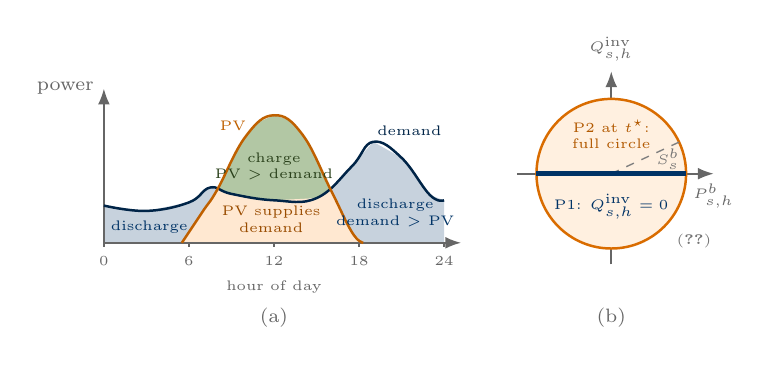
\begin{tikzpicture}[
    x=0.18cm,
    y=1.35cm,
    font=\footnotesize,
    >=Latex
]

% =============================================================
% (a) Daily demand, PV generation, and BESS operation
% =============================================================

% PV-surplus region: PV exceeds demand and the BESS charges
\fill[mygreen!45]
    (8.0,0.50)
    -- (9,0.78)
    -- (10,1.00)
    -- (11,1.14)
    -- (12,1.20)
    -- (13,1.16)
    -- (14,1.02)
    -- (15,0.78)
    -- (16,0.50)
    -- (15,0.42)
    -- (14,0.41)
    -- (13,0.40)
    -- (12,0.40)
    -- (11,0.41)
    -- (10,0.43)
    -- (9,0.46)
    -- cycle;

% Morning deficit: demand exceeds PV and the BESS discharges
\fill[execBlue!22]
    (0,0.35)
    -- (3,0.30)
    -- (6,0.38)
    -- (7.5,0.52)
    -- (8,0.50)
    -- (7,0.30)
    -- (5.5,0)
    -- (0,0)
    -- cycle;

% Evening deficit: demand exceeds PV and the BESS discharges
\fill[execBlue!22]
    (16,0.49)
    -- (17.5,0.72)
    -- (19,0.95)
    -- (21,0.80)
    -- (23,0.45)
    -- (24,0.40)
    -- (24,0)
    -- (18.3,0)
    -- (17.5,0.10)
    -- (16.5,0.38)
    -- cycle;

% Direct PV supply: min(PV generation, demand)
\fill[orange!18]
    (5.5,0)
    -- (7,0.30)
    -- (8,0.50)
    -- (9,0.46)
    -- (12,0.40)
    -- (15,0.42)
    -- (16,0.49)
    -- (16.5,0.38)
    -- (17.5,0.10)
    -- (18.3,0)
    -- cycle;

\node[
    font=\tiny,
    text=orange!60!black,
    align=center
] at (11.8,0.22)
{PV supplies\\demand};

% Axes
\draw[
    ->,
    black!60,
    line width=0.6pt
]
(0,0) -- (25.2,0);

\draw[
    ->,
    black!60,
    line width=0.6pt
]
(0,0) -- (0,1.45)
node[left, font=\scriptsize] {power};

% Time ticks
\foreach \x in {0,6,12,18,24}{
    \draw[
        black!60,
        line width=0.5pt
    ]
    (\x,0) -- (\x,-0.04);

    \node[
        below,
        font=\tiny,
        text=black!60
    ] at (\x,-0.04) {\x};
}

\node[
    font=\tiny,
    text=black!60
] at (12,-0.42)
{hour of day};

% Demand curve
\draw[
    execBlue!70!black,
    line width=0.9pt
]
plot[
    smooth,
    tension=0.7
]
coordinates {
    (0,0.35)
    (3,0.30)
    (6,0.38)
    (7.5,0.52)
    (9,0.46)
    (12,0.40)
    (15,0.42)
    (17.5,0.72)
    (19,0.95)
    (21,0.80)
    (23,0.45)
    (24,0.40)
};

% PV-generation curve
\draw[
    orange!75!black,
    line width=0.9pt
]
plot[
    smooth,
    tension=0.7
]
coordinates {
    (5.5,0.0)
    (7,0.30)
    (8,0.50)
    (10,1.00)
    (12,1.20)
    (14,1.02)
    (16,0.50)
    (17.5,0.10)
    (18.3,0.0)
};

% Curve labels
\node[
    font=\tiny,
    text=orange!75!black,
    anchor=west
] at (7.5,1.10)
{PV};

\node[
    font=\tiny,
    text=execBlue!70!black,
    anchor=west
] at (18.6,1.05)
{demand};

% Operating-region labels
\node[
    font=\tiny,
    text=mygreen!50!black,
    align=center
] at (12,0.72)
{charge\\PV \(>\) demand};

\node[
    font=\tiny,
    text=execBlue,
    align=center
] at (20.55,0.28)
{discharge\\demand \(>\) PV};

\node[
    font=\tiny,
    text=execBlue
] at (3.2,0.15)
{discharge};

\node[
    font=\scriptsize,
    text=black!60
] at (12,-0.70)
{(a)};


% =============================================================
% (b) BESS inverter capability
% =============================================================

\begin{scope}[
    shift={(35.8,0.65)},
    x=1cm,
    y=1cm
]

% Active-power axis
\draw[
    ->,
    black!60,
    line width=0.6pt
]
(-1.2,0) -- (1.3,0)
node[below, font=\tiny] {\(P^{b}_{s,h}\)};

% Reactive-power axis
\draw[
    ->,
    black!60,
    line width=0.6pt
]
(0,-1.15) -- (0,1.3)
node[above, font=\tiny] {\(Q^{\mathrm{inv}}_{s,h}\)};

% Inverter capability region
\fill[orange!12]
    (0,0) circle (0.95);

\draw[
    orange!85!black,
    line width=0.9pt
]
(0,0) circle (0.95);

% Apparent-power radius
\draw[
    dashed,
    black!50,
    line width=0.5pt
]
(0,0) -- (25:0.95);

\node[
    font=\tiny,
    text=black!55
] at (0.72,0.18)
{\(S^{b}_{s}\)};

% Unity-power-factor operating line used by P1
\draw[
    execBlue,
    line width=1.6pt
]
(-0.95,0) -- (0.95,0);

\node[
    font=\tiny,
    text=execBlue,
    align=center
] at (0,-0.42)
{P1: \(Q^{\mathrm{inv}}_{s,h}=0\)};

\node[
    font=\tiny,
    text=orange!70!black,
    align=center
] at (0,0.50)
{P2 at \(t^\star\):\\full circle};

\node[
    font=\tiny,
    text=black!55
] at (1.05,-0.85)
{\eqref{eq:scircle}};

\node[
    font=\scriptsize,
    text=black!60
] at (0,-1.83)
{(b)};

\end{scope}

\end{tikzpicture}

\caption{BESS operation in the two optimization problems. (a)~Typical prosumer demand \(P^{d}_{s,h}\) and PV generation \(P^{g}_{s,h}\) over one day. Under self-consumption, PV generation supplies the local demand, the BESS charges during a PV surplus, and discharges during a PV deficit, reducing the residual exchange with the network. (b)~Inverter capability defined by~\eqref{eq:scircle}. P1 operates along the \(Q^{\mathrm{inv}}_{s,h}=0\) diameter, whereas P2 may use the complete \(P\)--\(Q\) capability during the flexibility slot \(h=t^\star\).}
\label{fig:profiles}

\end{figure}

Let \(E^{b}_{s,0}\) denote the BESS energy at the beginning of the optimization window. The energy at the end of slot \(h\) is

\begin{equation}
\label{eq:soc_dynamics}
\begin{aligned}
E^{b}_{s,h}
=
E^{b}_{s,0}
+
\Delta t
\sum_{\tau=1}^{h}
\left(
\eta^{b,+}_{s}P^{b,+}_{s,\tau}
-
\frac{P^{b,-}_{s,\tau}}{\eta^{b,-}_{s}}
\right),
\end{aligned}
\end{equation}

where \(\eta^{b,+}_{s}\) and \(\eta^{b,-}_{s}\) are the charging and discharging efficiencies, respectively, and \(\Delta t=0.5\)~h.

The BESS energy, power, and terminal-state limits are

\begin{subequations}
\label{eq:battery_limits}
\begin{align}
\underline{E}^{b}_{s}
\leq E^{b}_{s,h}
&\leq
\overline{E}^{b}_{s},
\label{eq:energy_limits}
\\
0
\leq P^{b,+}_{s,h},\,P^{b,-}_{s,h}
&\leq
\overline{P}^{b}_{s},
\label{eq:power_limits}
\\
-\varepsilon^{E}\overline{E}^{b}_{s}
\leq E^{b}_{s,H}-E^{b}_{s,0}
&\leq
\varepsilon^{E}\overline{E}^{b}_{s}.
\label{eq:terminal_band}
\end{align}
\end{subequations}

where \eqref{eq:terminal_band} limits the net energy deviation over the window and prevents end-of-horizon depletion.

The BESS inverter capability is constrained by

\begin{equation}
\label{eq:scircle}
\left(P^{b}_{s,h}\right)^2
+
\left(Q^{\mathrm{inv}}_{s,h}\right)^2
\leq
\left(S^{b}_{s}\right)^2,
\qquad
\forall s\in\mathcal{S},\ h\in\mathcal{H},
\end{equation}

where \(Q^{\mathrm{inv}}_{s,h}\) denotes the inverter reactive power and \(S^{b}_{s}\) its apparent-power rating. 

% ---------------------------------------------------------------------
\subsubsection{Three-Phase Network Model}
\label{ssec:three_phase_network}
% ---------------------------------------------------------------------

The network constraints are adopted from the convexified three-phase AC OPF formulation developed in~\cite{gutierrez2021,gutierrez2019} and are not reproduced in full here. 

In brief, the model represents phase voltages and currents in rectangular coordinates, includes mutual coupling between phases, and accounts for the fixed tap Dy11 transformer. Constant-power injections and the minimum-voltage constraint are linearized around a reference voltage profile that incorporates the MV--LV phase displacement.

The BESS decisions are coupled to the network currents through

\begin{subequations}
\label{eq:battery_current_power}
\begin{align}
P^{b}_{s,h}
&=
V^{\mathrm{re},0}_{n,\phi,h}I^{b,\mathrm{re}}_{s,h}
+
V^{\mathrm{im},0}_{n,\phi,h}I^{b,\mathrm{im}}_{s,h},
\label{eq:pbatt}
\\
Q^{\mathrm{inv}}_{s,h}
&=
V^{\mathrm{im},0}_{n,\phi,h}I^{b,\mathrm{re}}_{s,h}
-
V^{\mathrm{re},0}_{n,\phi,h}I^{b,\mathrm{im}}_{s,h}.
\label{eq:qbatt}
\end{align}
\end{subequations}

The PCC exchange used in the P2 objective is

\begin{subequations}
\label{eq:pcc_exchange}
\begin{align}
P^{\mathrm{PCC}}_{h}
&=
\sum_{\phi\in\Phi}
\left(
V^{\mathrm{re}}_{n_0,\phi}I^{\mathrm{re}}_{n_0,\phi,h}
+
V^{\mathrm{im}}_{n_0,\phi}I^{\mathrm{im}}_{n_0,\phi,h}
\right),
\label{eq:ppcc}
\\
Q^{\mathrm{PCC}}_{h}
&=
\sum_{\phi\in\Phi}
\left(
V^{\mathrm{im}}_{n_0,\phi}I^{\mathrm{re}}_{n_0,\phi,h}
-
V^{\mathrm{re}}_{n_0,\phi}I^{\mathrm{im}}_{n_0,\phi,h}
\right),
\label{eq:qpcc}
\end{align}
\end{subequations}

where \(n_0\) denotes the fixed voltage PCC bus and positive \(P^{\mathrm{PCC}}_{h}\) denotes import. The reachable FOR is constructed from these exchanges at \(h=t^\star\).

The OPF enforces the branch-current and voltage limits

\begin{subequations}
\label{eq:network_limits}
\begin{align}
\left(I^{\mathrm{re}}_{e,\phi,h}\right)^2
+
\left(I^{\mathrm{im}}_{e,\phi,h}\right)^2
&\leq
\overline{I}_{e}^{\,2},
\label{eq:thermal}
\\
\left(V^{\mathrm{re}}_{n,\phi,h}\right)^2
+
\left(V^{\mathrm{im}}_{n,\phi,h}\right)^2
&\leq
\overline{V}_{n}^{\,2},
\label{eq:vmax}
\\
2V^{\mathrm{re},0}_{n,\phi,h}V^{\mathrm{re}}_{n,\phi,h}
+
2V^{\mathrm{im},0}_{n,\phi,h}V^{\mathrm{im}}_{n,\phi,h}
-
\left|V^{0}_{n,\phi,h}\right|^{2}
&\geq
\underline{V}_{n}^{\,2}.
\label{eq:vmin}
\end{align}
\end{subequations}

```latex
% ---------------------------------------------------------------------
\subsection{Network-Constrained Self-Consumption Dispatch (P1)}
\label{ssec:selfconsumption}
% ---------------------------------------------------------------------
P1 computes a network-feasible self-consumption schedule and determines the BESS action implemented at the current slot \(h=1\). Local PV generation supplies demand, surplus generation may charge the BESS, and stored energy may be discharged to reduce grid imports.

Over the common feasible set \(\mathcal{X}_{k}\), P1 minimizes prosumer grid exchange and BESS throughput:

\begin{equation}
\label{eq:Jsc}
\begin{aligned}
J^{\mathrm{sc}}
={}&
\sum_{s\in\mathcal{S}}
\sum_{h\in\mathcal{H}\setminus\{t^\star\}}
\omega^{\mathrm{self}}_{h}
\left(
P^{+}_{s,h}+P^{-}_{s,h}
\right)
\\
&+
\mu
\sum_{s\in\mathcal{S}}
\sum_{h\in\mathcal{H}}
\left(
P^{b,+}_{s,h}+P^{b,-}_{s,h}
\right).
\end{aligned}
\end{equation}

The first term promotes self-consumption. Since

\begin{equation}
\label{eq:exchange_split_identity}
P_{s,h}=P^{+}_{s,h}-P^{-}_{s,h},
\qquad
P^{+}_{s,h},P^{-}_{s,h}\geq0,
\end{equation}

minimizing \(P^{+}_{s,h}+P^{-}_{s,h}\) reduces \(\lvert P_{s,h}\rvert\), and therefore both imports and exports whenever they can be offset by local PV generation and BESS operation.

The flexibility slot \(h=t^\star\) is excluded from this term to avoid biasing the PCC exchange explored by P2. All device, energy, and network constraints remain enforced at this slot.

The second term penalizes BESS throughput, discouraging unnecessary cycling and simultaneous charging and discharging while preserving a continuous convex formulation. The coefficient \(\mu\) is selected to make loss-driven charge--discharge cycles unattractive and is reported in Section~\ref{sec:case}.

At rolling step \(k\), P1 is formulated as

\begin{subequations}
\label{eq:P1}
\begin{align}
\text{(P1)}\qquad
\min_{\bm{x}_{k}}\quad
& J^{\mathrm{sc}},
\label{eq:P1_obj}
\\
\text{s.t.}\quad
& \bm{x}_{k}\in\mathcal{X}_{k},
\label{eq:P1_common}
\\
& Q^{\mathrm{inv}}_{s,h}=0,
\quad
\forall s\in\mathcal{S},\
h\in\mathcal{H}.
\label{eq:P1_qzero}
\end{align}
\end{subequations}

Constraint~\eqref{eq:P1_qzero} disables BESS reactive-power support during the baseline dispatch.

Only the current-slot setpoints

\begin{equation}
\label{eq:P1_committed_actions}
\left(
\widehat{P}^{b,+}_{s,1\mid k},
\widehat{P}^{b,-}_{s,1\mid k}
\right)
\end{equation}

are implemented. The decisions for \(h\geq2\) ensure a feasible continuation over the remaining horizon. P2 fixes the implemented action and computes the reachable PCC exchanges at \(h=t^\star\).


\subsection{Next-Interval Reachable FOR Construction (P2)} \label{ssec:for_next_interval}

P2 constructs the network-feasible PCC exchanges available at the target slot \(h=t^\star\), conditioned on the current-slot BESS action committed by P1. The directional search set is 

\begin{equation} 
\label{eq:directions} 
\Theta = \left\{ \theta_i=\frac{2\pi i}{N_\theta} \;\middle|\; i=0,\ldots,N_\theta-1 \right\}. 
\end{equation} 

For each \(\theta_i\in\Theta\), P2 solves 

\begin{subequations} 
\label{eq:P2} \begin{align} \text{(P2)}\qquad \max_{\bm{x}_{k,i}}\quad & P^{\mathrm{PCC}}_{t^\star\mid k,i}\cos\theta_i + Q^{\mathrm{PCC}}_{t^\star\mid k,i}\sin\theta_i, \label{eq:P2_obj} \\ \text{s.t.}\quad & \bm{x}_{k,i}\in\mathcal{X}_{k}, \label{eq:P2_common} \\ & P^{b,+}_{s,1\mid k,i} = \widehat{P}^{b,+}_{s,1\mid k}, \quad \forall s\in\mathcal{S}, \label{eq:P2_chg} \\ & P^{b,-}_{s,1\mid k,i} = \widehat{P}^{b,-}_{s,1\mid k}, \quad \forall s\in\mathcal{S}, \label{eq:P2_dis} \\ & Q^{\mathrm{inv}}_{s,h\mid k,i}=0, \quad \forall s\in\mathcal{S},\ h\in\mathcal{H}\setminus\{t^\star\}. \label{eq:P2_q} 
\end{align} 
\end{subequations} 

The objective traces a PCC boundary point in the direction \(\theta_i\). Constraints~\eqref{eq:P2_chg} and~\eqref{eq:P2_dis} fix the P1 action, ensuring that all directional solves enter the target slot from the same post-dispatch BESS state.  The Constraint~\eqref{eq:P2_q} restricts the reactive power support to \(h=t^\star\), while all constraints in \(\mathcal{X}_{k}\) remain enforced throughout the horizon. Figure~\ref{fig:p2_zoom_match} illustrates this construction.


\begin{figure}[h!]
\centering
% ============================ KNOBS ============================
\def\pTwoScale{1.00}
\colorlet{p2Exec}{execBlue}
\definecolor{p2FOR}{RGB}{224,138,30}
\colorlet{p2Region}{p2FOR}
\colorlet{p2Batt}{mygreen}
% ==============================================================

\resizebox{\pTwoScale\columnwidth}{!}{%
\begin{tikzpicture}[
    font=\footnotesize,
    >=Latex,
    pcell/.style={
        draw=black!40,
        line width=0.5pt,
        minimum width=0.6cm,
        minimum height=0.6cm,
        anchor=south west,
        inner sep=1pt,
        align=center,
        font=\scriptsize
    },
    ex/.style={
        pcell,
        fill=p2Exec!30,
        draw=p2Exec,
        line width=0.9pt
    },
    fo/.style={
        pcell,
        fill=p2FOR!32,
        draw=p2FOR!80!black,
        line width=0.9pt
    },
    lbl/.style={
        font=\tiny,
        text=black!60,
        align=center
    },
    note/.style={
        font=\tiny,
        align=center,
        inner sep=1.5pt
    },
    qnode/.style={
        circle,
        fill=black!65,
        draw=white,
        line width=0.25pt,
        minimum size=3.5pt,
        inner sep=0pt
    }
]

% ==============================================================
% Band 1: title
% ==============================================================

\node[
    anchor=west,
    font=\scriptsize\bfseries,
    text=textGray
] at (0,1.60)
{zoom of the P2 construction at step $k=20$};

% ==============================================================
% Band 2: operation and flexibility slots
% ==============================================================

\node[
    font=\tiny\bfseries,
    text=p2Exec
] at (0.30,0.84)
{$h{=}1$};

\node[
    font=\tiny\bfseries,
    text=p2FOR!85!black
] at (1.20,0.84)
{$h{=}2{=}t^\star$};

\node[ex] at (0.00,0) {20};
\node[fo] at (0.66,0) {21};

% P1 connection
\draw[
    ->,
    p2Exec,
    line width=0.8pt
]
(0.30,-1.00) -- (0.30,-0.05);

\node[
    font=\tiny\bfseries,
    text=p2Exec,
    anchor=east
] at (0.02,-0.50)
{P1};

% P2 connection
\draw[
    ->,
    p2FOR!85!black,
    line width=0.8pt
]
(0.96,-0.05) -- (2.10,-0.78);

\node[
    font=\tiny\bfseries,
    text=p2FOR!85!black
] at (1.72,-0.28)
{P2};

% ==============================================================
% P1 mini-house with PV and battery
% ==============================================================

\begin{scope}[shift={(0.30,-1.35)}]

    % House body
    \draw[
        line width=0.6pt,
        draw=black!55,
        fill=p2Exec!10
    ]
    (-0.16,-0.18) rectangle (0.16,0.05);

    % House roof
    \draw[
        line width=0.6pt,
        draw=black!55,
        fill=p2Exec!18
    ]
    (-0.20,0.05) --
    (0,0.24) --
    (0.20,0.05) --
    cycle;

    % PV panel
    \draw[
        line width=0.4pt,
        draw=p2Exec,
        fill=p2Exec!50
    ]
    (-0.13,0.09) --
    (-0.02,0.185) --
    (0.03,0.15) --
    (-0.08,0.055) --
    cycle;

    % Battery
    \draw[
        line width=0.5pt,
        draw=p2Batt!70!black,
        fill=p2Batt!35
    ]
    (-0.055,-0.14) rectangle (0.065,-0.02);

    % Battery terminal
    \draw[
        line width=0.6pt,
        draw=p2Batt!70!black
    ]
    (0.005,-0.02) -- (0.005,0.002);

\end{scope}

\node[
    font=\tiny,
    text=p2Exec,
    align=center
] at (0.30,-1.92)
{commit $\widehat{P}^{b,\pm}_{s,1|20}$};

% ==============================================================
% Committed battery state
% ==============================================================

\draw[
    ->,
    p2Exec!80!black,
    line width=0.7pt
]
(0.84,-1.35) -- (1.92,-1.35);

\node[
    font=\tiny,
    text=p2Exec!80!black
] at (1.25,-1.16)
{$\widehat E^{b}_{s,1|20}$};

% ==============================================================
% Enlarged P2 directional construction
% ==============================================================

\begin{scope}[shift={(4.80,-1.20)}]

% PCC axes
\draw[
    ->,
    black!45,
    line width=0.45pt
]
(-1.95,0) -- (2.15,0)
node[
    right,
    font=\scriptsize,
    inner sep=1pt
]
{$P^{\mathrm{PCC}}$};

\draw[
    ->,
    black!45,
    line width=0.45pt
]
(0,-1.45) -- (0,1.60)
node[
    above,
    font=\scriptsize,
    inner sep=1pt
]
{$Q^{\mathrm{PCC}}$};

% Polygonal reachable FOR
\fill[
    p2Region!22,
    draw=p2Region!85!black,
    line width=0.7pt
]
( 1.35, 0.58) --
( 1.75, 0.02) --
( 1.46,-0.62) --
( 0.78,-1.02) --
( 0.00,-1.20) --
(-0.82,-1.04) --
(-1.45,-0.58) --
(-1.72, 0.02) --
(-1.47, 0.60) --
(-0.95, 1.02) --
(-0.14, 1.24) --
( 0.66, 1.04) --
cycle;

% Directional rays and support points
\foreach \x/\y in {
     1.35/0.58,
     1.75/0.02,
     1.46/-0.62,
     0.78/-1.02,
     0.00/-1.20,
    -0.82/-1.04,
    -1.45/-0.58,
    -1.72/0.02,
    -1.47/0.60,
    -0.95/1.02,
    -0.14/1.24,
     0.66/1.04
}{
    \draw[
        dashed,
        draw=black!32,
        line width=0.38pt,
        ->
    ]
    (0,0) -- (\x,\y);

    \node[qnode] at (\x,\y) {};
}

% Selected search direction
\draw[
    ->,
    p2FOR!90!black,
    line width=1.0pt
]
(0,0) -- (1.86,0.80);

% Selected support point
\fill[p2FOR!90!black]
(1.35,0.58) circle (2.0pt);

% Directional support line
\draw[
    draw=red!70!black,
    line width=0.8pt
]
($(1.35,0.58)+(-0.42,0.92)$) --
($(1.35,0.58)+(0.42,-0.92)$);

% Direction label
\node[
    note,
    text=p2FOR!90!black,
    fill=white,
    anchor=west
] at (1.56,0.92)
{$\mathbf d_{\theta_i}$};

% Support-point label
\node[
    note,
    text=red!70!black,
    fill=white,
    anchor=east
] at (1.58,1.70)
{$\mathbf y^\star_{20,i}$};

% Reachable-FOR label
\node[
    font=\tiny\bfseries,
    text=p2Region!85!black,
    align=center
] at (-1.95,0.30)
{$\widehat{\mathcal F}^{\,\mathrm R}_{20}$};

% Number of search directions
\node[
    note,
    text=black!55,
    anchor=west
] at (-1.88,1.34)
{$N_\theta=12$};

\end{scope}

\node[
    font=\tiny,
    text=p2FOR!85!black,
    align=center
] at (4.80,-3.05)
{directional sweep at the flexibility slot};

\end{tikzpicture}%
}

\caption{P2 construction at rolling step \(k=20\). P1 commits the
operation-slot BESS powers
\(\widehat{P}^{b,\pm}_{s,1\mid 20}\), determining the energy state
\(\widehat{E}^{b}_{s,1\mid 20}\) entering the flexibility slot
\(h=t^\star\). P2 solves \(N_{\theta}=12\) directional OPFs, and the
convex hull of the resulting boundary points \(\bm{y}^{\star}_{20,i}\) defines the reachable FOR
\(\widehat{\mathcal{F}}^{\mathrm{R}}_{20}\).}
\label{fig:p2_zoom_match}
\end{figure}

The optimal PCC exchange obtained in direction \(\theta_i\) is 

\begin{equation} 
\label{eq:P2_boundary_point} \bm{y}^{\star}_{k,i} = \begin{bmatrix} P^{\mathrm{PCC},\star}_{t^\star\mid k,i} \\[1mm] Q^{\mathrm{PCC},\star}_{t^\star\mid k,i} \end{bmatrix}, \end{equation} 

and the polygonal reachable FOR is 

\begin{equation} 
\label{eq:FOR_polygon} \widehat{\mathcal{F}}_{k}^{\,\mathrm{R}} = \operatorname{conv} \left\{ \bm{y}^{\star}_{k,i} \;\middle|\; i=0,\ldots,N_\theta-1 \right\}. 
\end{equation} 

Each boundary point is supported by a feasible full-horizon trajectory consistent with the P1 action. Moreover, because \(\mathcal{X}_{k}\) is convex, the commitment constraints are affine, and the PCC exchange is linear, the interior of \(\widehat{\mathcal{F}}_{k}^{\,\mathrm{R}}\) is also reachable. For finite \(N_\theta\), the polygon provides an inner approximation of the complete reachable FOR. 

% use section* for acknowledgment
\section*{Acknowledgment}


The authors would like to thank...

\bibliographystyle{IEEEtran}
\bibliography{refs_paper1}

% Placeholder biography; switch back to \begin{IEEEbiography}[{\includegraphics[width=1in,height=1.25in,clip,keepaspectratio]{foto_autor.png}}]{...} once author photos are available.
\begin{IEEEbiographynophoto}{Nombre Autor}
Texto de la biografía aquí...

%repeat for other authors

\end{IEEEbiographynophoto}

\end{document}

